%%%%%%%%%%%%%%%%%%%%%%%%%%%%%%%%%%%%%%%%%
% Short Sectioned Assignment LaTeX Template Version 1.0 (5/5/12)
% This template has been downloaded from: http://www.LaTeXTemplates.com
% Original author:  Frits Wenneker (http://www.howtotex.com)
% License: CC BY-NC-SA 3.0 (http://creativecommons.org/licenses/by-nc-sa/3.0/)
%%%%%%%%%%%%%%%%%%%%%%%%%%%%%%%%%%%%%%%%%

%----------------------------------------------------------------------------------------
%	PACKAGES AND OTHER DOCUMENT CONFIGURATIONS
%----------------------------------------------------------------------------------------

\documentclass[paper=a4, fontsize=11pt]{scrartcl} % A4 paper and 11pt font size

% ---- Entrada y salida de texto -----

\usepackage{hyperref}
\usepackage{varioref}
\usepackage[T1]{fontenc} % Use 8-bit encoding that has 256 glyphs
\usepackage[utf8]{inputenc}
%\usepackage{fourier} % Use the Adobe Utopia font for the document - comment this line to return to the LaTeX default

% ---- Idioma --------

\usepackage[spanish, es-tabla]{babel} % Selecciona el español para palabras introducidas automáticamente, p.ej. "septiembre" en la fecha y especifica que se use la palabra Tabla en vez de Cuadro

% ---- Otros paquetes ----

\usepackage{amsmath,amsfonts,amsthm} % Math packages
%\usepackage{graphics,graphicx, floatrow} %para incluir imágenes y notas en las imágenes
\usepackage{graphics,graphicx, float} %para incluir imágenes y colocarlas

% Para hacer tablas comlejas
%\usepackage{multirow}
%\usepackage{threeparttable}

%\usepackage{sectsty} % Allows customizing section commands
%\allsectionsfont{\centering \normalfont\scshape} % Make all sections centered, the default font and small caps

\usepackage{fancyhdr} % Custom headers and footers
\pagestyle{fancyplain} % Makes all pages in the document conform to the custom headers and footers
\fancyhead{} % No page header - if you want one, create it in the same way as the footers below
\fancyfoot[L]{} % Empty left footer
\fancyfoot[C]{} % Empty center footer
\fancyfoot[R]{\thepage} % Page numbering for right footer
\renewcommand{\headrulewidth}{0pt} % Remove header underlines
\renewcommand{\footrulewidth}{0pt} % Remove footer underlines
\setlength{\headheight}{13.6pt} % Customize the height of the header

\numberwithin{equation}{section} % Number equations within sections (i.e. 1.1, 1.2, 2.1, 2.2 instead of 1, 2, 3, 4)
\numberwithin{figure}{section} % Number figures within sections (i.e. 1.1, 1.2, 2.1, 2.2 instead of 1, 2, 3, 4)
\numberwithin{table}{section} % Number tables within sections (i.e. 1.1, 1.2, 2.1, 2.2 instead of 1, 2, 3, 4)

\setlength\parindent{0pt} % Removes all indentation from paragraphs - comment this line for an assignment with lots of text

\newcommand{\horrule}[1]{\rule{\linewidth}{#1}} % Create horizontal rule command with 1 argument of height


%----------------------------------------------------------------------------------------
%	TÍTULO Y DATOS DEL ALUMNO
%----------------------------------------------------------------------------------------

\title{	
\normalfont \normalsize 
\textsc{{\bf Ingeniería de Servidores (2015-2016)} \\ Grado en Ingeniería Informática \\ Universidad de Granada} \\ [25pt] % Your university, school and/or department name(s)
\horrule{0.5pt} \\[0.4cm] % Thin top horizontal rule
\huge Memoria Práctica 5 \\ % The assignment title
\horrule{2pt} \\[0.5cm] % Thick bottom horizontal rule
}

\author{Francisco Carrillo Pérez} % Nombre y apellidos

\date{\normalsize\today} % Incluye la fecha actual

%----------------------------------------------------------------------------------------
% DOCUMENTO
%----------------------------------------------------------------------------------------

\begin{document}

\maketitle % Muestra el Título

\newpage %inserta un salto de página

\tableofcontents % para generar el índice de contenidos

\listoffigures

\listoftables

\newpage

%%%%%%%%%%%%%%%%%%%%%%%%%%%%%%%%%%%%%%%%%%%%%%%%%%%%
% CUESTIÓN 1
%%%%%%%%%%%%%%%%%%%%%%%%%%%%%%%%%%%%%%%%%%%%%%%%%%%%

\section{Cuestión 1: Al modificar los valores del kernel de este modo, no logramos que persistan después de reiniciar la máquina. ¿Qué archivo hay que editar para que los cambios sean permanentes?}

Para modificar los valores del kernel y conseguir que persistan después de reiniciar debemos editar también el archivo \textbf{/etc/sysctl.conf } \cite{systcl1} . Un ejemplo de uso sería:

\begin{itemize}
	\item Vamos a cambiar el valor de cuento tiempo es necesario que un proceso esté ejecutándose para que el CFS decida cambiarlo a otro core. Para ello primero ejecutamos el comando \textbf{sudo sysctl -w kernel.sched\_migration\_cost\_ns=5000000}. Podemos ver el resultado en la Figura \ref{figura1}.
	\item Ahora añadimos la misma línea, \textbf{kernel.sched\_migration\_cost\_ns=5000000}, al archivo /etc/sysctl.conf . Podemos observar el resultado en la Figura \ref{figura2}
	\item Y por último hacemos un \textbf{sudo sysctl -p} para que se guarden los cambios. Podemos observar el resultado en la Figura \ref{figura3}.
\end{itemize}
\begin{figure}[H] %con el [H] le obligamos a situar aquí la figura
	\centering
	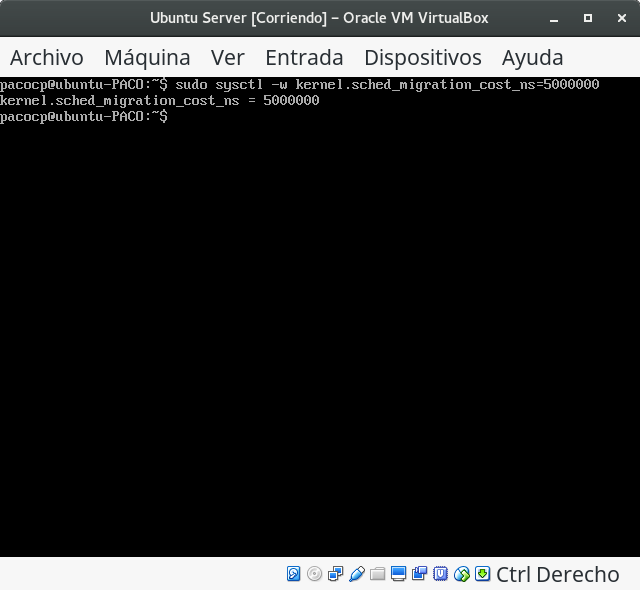
\includegraphics[scale=0.5]{figuras/figura1.png}  %el parámetro scale permite agrandar o achicar la imagen. En el nombre de archivo puede especificar directorios
	
	
	\caption{Resultado al ejecutar \textbf{sudo sysctl -w kernel.sched\_migration\_cost\_ns=5000000}}
	\label{figura1}
\end{figure}
\begin{figure}[H] %con el [H] le obligamos a situar aquí la figura
	\centering
	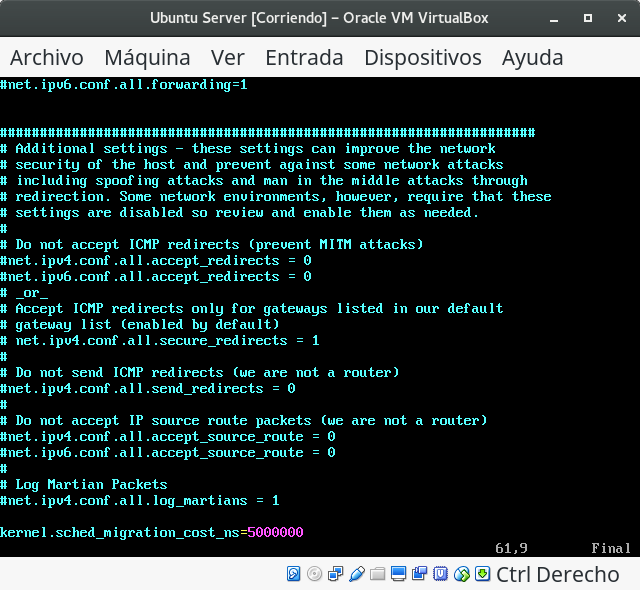
\includegraphics[scale=0.5]{figuras/figura2.png}  %el parámetro scale permite agrandar o achicar la imagen. En el nombre de archivo puede especificar directorios
	
	
	\caption{Modificamos el archivo /etc/sysctl.conf y añadimos la línea \textbf{kernel.sched\_migration\_cost\_ns=5000000}}
	\label{figura2}
\end{figure}
\begin{figure}[H] %con el [H] le obligamos a situar aquí la figura
	\centering
	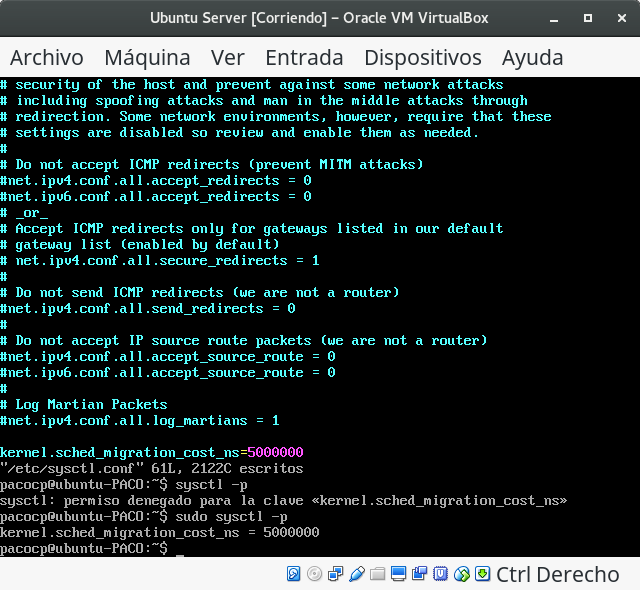
\includegraphics[scale=0.5]{figuras/figura3.png}  %el parámetro scale permite agrandar o achicar la imagen. En el nombre de archivo puede especificar directorios
	
	
	\caption{Guardamos los cambios con el comando \textbf{sudo susctl -p}}
	\label{figura3}
\end{figure}

%%%%%%%%%%%%%%%%%%%%%%%%%%%%%%%%%%%%%%%%%%%%%%%%%%%%
% CUESTIÓN 2
%%%%%%%%%%%%%%%%%%%%%%%%%%%%%%%%%%%%%%%%%%%%%%%%%%%%

\section{Cuestión 2: ¿Con qué opción se muestran todos los parámetros modificables en tiempo de ejecución? Elija dos parámetros y expliqué, en dos líneas, qué función tienen.}

Consultando el man de sysctl \cite{sysctl2} podemos observar que con la opción -a podemos ver todos los parámetros modificables en tiempo de ejecución.

\begin{enumerate}
	\item La variable \textbf{fs.file-max} nos permite modificar el número máximo de archivos que un proceso puede abrir.
	\item La variable \textbf{net.ipv4.ip\_local\_port\_range} nos permite modificar el rango de puertos que podemos usar, por ejemplo podríamos poner net.ipv4.ip\_local\_port\_range = 1024 65535 para que usara todo el rango de puertos.
\end{enumerate}

%%%%%%%%%%%%%%%%%%%%%%%%%%%%%%%%%%%%%%%%%%%%%%%%%%%%
% CUESTIÓN 3
%%%%%%%%%%%%%%%%%%%%%%%%%%%%%%%%%%%%%%%%%%%%%%%%%%%%

\section{Cuestión 3: Realice una copia de seguridad del registro y restaurela, ilustre el proceso con capturas.}

%%%%%%%%%%%%%%%%%%%%%%%%%%%%%%%%%%%%%%%%%%%%%%%%%%%%
% CUESTIÓN 4
%%%%%%%%%%%%%%%%%%%%%%%%%%%%%%%%%%%%%%%%%%%%%%%%%%%%

\section{Cuestión 4:}

\subsection{¿Cómo se abre una consola en Windows?}
Para abrir una consola simplemente buscamos \textbf{cmd}. Podemos observarlo en la Figura \ref{figura7}

\begin{figure}[H] %con el [H] le obligamos a situar aquí la figura
	\centering
	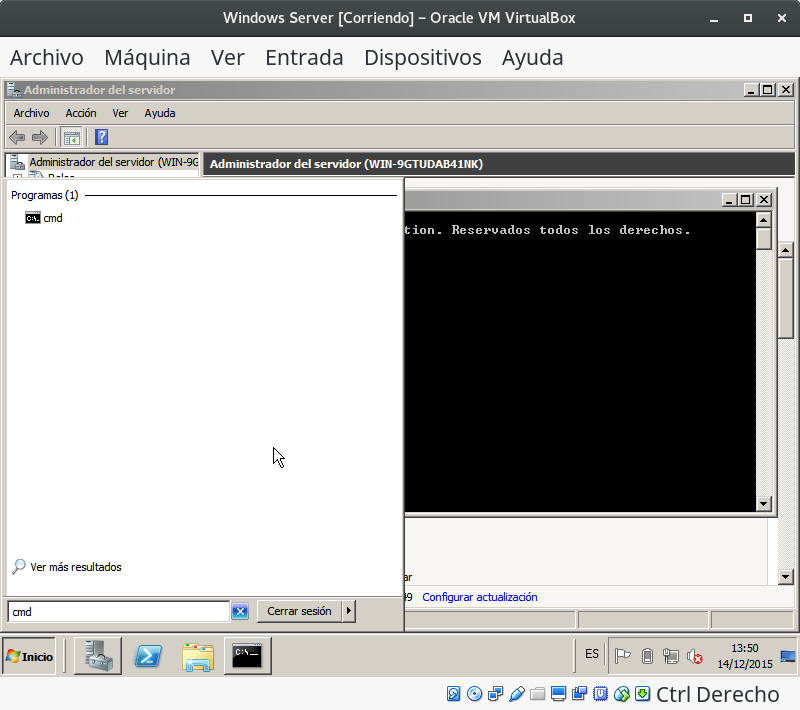
\includegraphics[scale=0.5]{figuras/figura7.png}  %el parámetro scale permite agrandar o achicar la imagen. En el nombre de archivo puede especificar directorios
	
	
	\caption{Consola en Windows Server}
	\label{figura7}
\end{figure}
\subsection{¿Qué comando hay que ejecutar para editar el registro? Muestre su ejecución con capturas de pantalla.}
%El comando que se utiliza para editar el registro es el comando \textbf{reg} \cite{reg}. Vamos a ejecutar el siguiente comando de la página de Microsoft . El comando es \textbf{REG ADD HKLM\textbackslashSoftware\textbackslashMyCo /v Data /t REG_BINARY /d fe340ead} y lo que realiza es añadir un registro a la entrada HKLM\textbackslashSoftware\textbackslashMyCo con un valor llamado Data, del tipo REG_BINARY, y con valor de datos fe340ead. Podemos observar que tiene resultado satisfactorio en la Figura \ref{figura8}

%\begin{figure}[H] %con el [H] le obligamos a situar aquí la figura
%	\centering
%	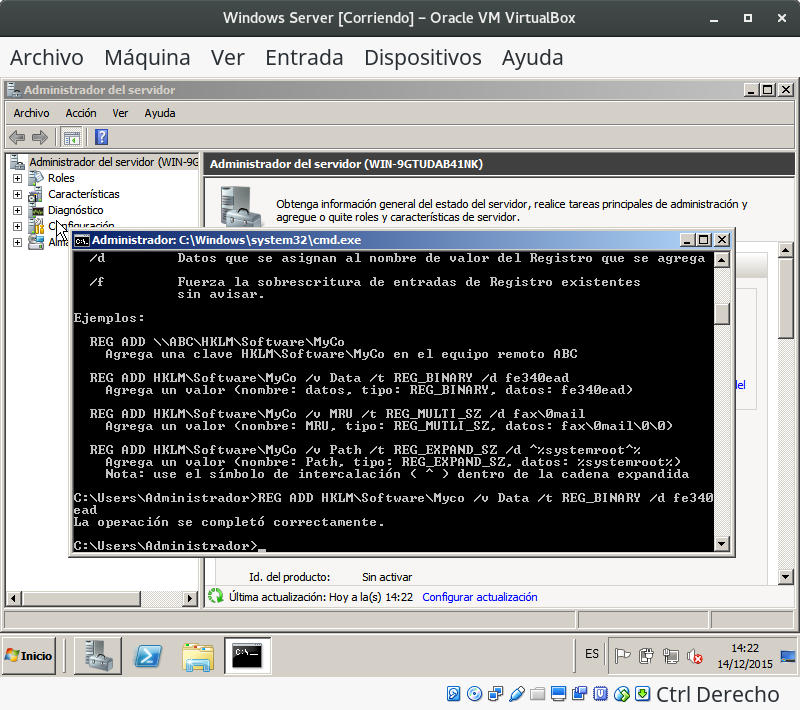
\includegraphics[scale=0.5]{figuras/figura8.png}  %el parámetro scale permite agrandar o achicar la imagen. En el nombre de archivo puede especificar directorios
	
	
%	\caption{Resultado de ejecutar el comando REG ADD HKLM\textbackslashSoftware\textbackslashMyCo /v Data /t REG_BINARY /d fe340ead}
%	\label{figura8}
%\end{figure}

%%%%%%%%%%%%%%%%%%%%%%%%%%%%%%%%%%%%%%%%%%%%%%%%%%%%
% CUESTIÓN 5
%%%%%%%%%%%%%%%%%%%%%%%%%%%%%%%%%%%%%%%%%%%%%%%%%%%%

\section{Cuestión 5: Las cadenas de caracteres y valores numéricos tienen distintos	tipos. Busque en la documentación de Microsoft y liste todos los tipos de valores.}

En la siguiente página podemos observar los distintos tipos \cite{registryvalues}:

%\begin{itemize}
%	\item \textbf{REG\_BINARY: } \textquotedblleft Datos binarios en cualquier forma.\textquotedblright
%	\item \textbf{REG\_DWORD: } \textquotedblleft Un número de 32 bits.\textquotedblright
%	\item \textbf{REG\_DWORD\_LITTLE_ENDIAN: } \textquotedblleft Un número de 32 bits en formato little endian.\textquotedblright
%	\item \textbf{REG\_DWORD_BIG_ENDIAN: } \textquotedblleft Un número de 32 bits en formato big endian.\textquotedblright
%	\item \textbf{REG\_EXPAND\_SZ: }\textquotedblleft Una cadena de caracteres que acaba en null que contiene referencias sin expandir a %variables locales.\textquotedblright
%	\item \textbf{REG\_LINK: }\textquotedblleft Una cadena de caracteres  que acaba en null que contiene el path que se da como argumento, %de un enlace simbólico que fue creado llamando a la función RegCreateKeyEx con REG_OPTION_CREATE_LINK.\textquotedblright
%	\item \textbf{REG\_MULTI_SZ: }\textquotedblleft Una secuencia de cadenas de caracteres que acaba en null que termina con una cadena %vacía.\textquotedblright
%	\item \textbf{REG\_NONE: }\textquotedblleft Ningún valor definido.\textquotedblright
%	\item \textbf{REG\_QWORD: }\textquotedblleft Un número de 64 bits.\textquotedblright
%	\item \textbf{REG\_QWORD\_LITTLE\_ENDIAN: }\textquotedblleft Un número de 64 bits en formato little endian.\textquotedblright
%	\item \textbf{REG\_SZ: }\textquotedblleft Una cadena de caracteres que acaba en null.\textquotedblright
%\end{itemize}


%%%%%%%%%%%%%%%%%%%%%%%%%%%%%%%%%%%%%%%%%%%%%%%%%%%%
% CUESTIÓN 6
%%%%%%%%%%%%%%%%%%%%%%%%%%%%%%%%%%%%%%%%%%%%%%%%%%%%

\section{Cuestión 6: Enumere qué elementos se pueden configurar en Apache y en IIS para que Moodle funcione mejor.}

Para ambos: 
\begin{itemize}
	\item Mejora el comportamiento de PHP cuando se instala como un módulo de Apache o ISS.
\end{itemize}

Para Apache:
\begin{itemize}
	\item Si estás utilizando Apache en Windows es mejor usar la versión de Apache Lounge que se ha comprobado que tiene mejoras a la versión oficial de Apache.
	\item Establecer la directiva de \textbf{MaxClients} de forma correcta. Hay que utilizar la siguiente regla:\\
	$MaxClients = \frac{Total available memory * 80\%}{Max memory usage of apache process}$
	\item Reducir en la mayor medida el número de módulos que carga apache en el archivo httpd.config.
	\item Usar la última versión de Apache.
	\item En Linux, reducir hasta entre 20 y 30 el número de \textbf{MaxRequestsPerChild} en el archivo httpd.config
	\item Para aquellos casos en los que se hace un uso intensivo del servidor, considerar el ajuste \textbf{KeepAlive Off} o reducir el valor de \textbf{KeepAliveTimeout} entre 2 y 5.
	\item Como una alternativa al ajuste \textbf{KeepAlive Off}, barajar la opción de usar un \textbf{Reverse Proxy server} en frente del servidor Moodle.
	\item Si no usas un archivo .htaccess, cambiar la variable  \textbf{AllowOverride} a AllowOverride None para prevenir que se pueda ver el archivo htaccess .
	\item Establecer el \textbf{DirectoryIndex} de forma correcta para evitar la negociación de contenido.
	\item A no ser que estes realizando trabajo de desarrollo en el servidor, establece \textbf{ExtendedStatus Off} y  mod\_info y también mod\_status.
	\item Deja \textbf{HostnameLookups Off } para reducir la latencia de DNS.
	\item Considerar reducir el  valor de \textbf{TimeOut} entre 30 y 60 segundos.
	\item En \textbf{Options directive}, evitar Options Multiviews ya que esto mejora un escaneo de directorio. Para reducir las I/O de disco mejor usar: \textbf{Options -Indexes FollowSymLinks} .
	\item \textbf{Caching} (solo si utilizas Moodle 1.9) 
\end{itemize}

Para ISS (Todo se altera esta localización en el registro: \textbf{}):
\begin{itemize}
	\item El equivalente a KeepAliveTimeout es \textbf{ListenBackLog}, establecerlo entre 2 y 5.
	\item Cambiar el valor de \textbf{MemCacheSize} para ajustar al valor de memoria caché que ISS utilizará.
	\item Cambiar el valor de \textbf{MaxCachedFileSize} para que se ajuste al máximo archivo en caché de la caché de archivos en bytes.
	\item Crear una nueva DWORD llamada \textbf{ ObjectCacheTTL} que permita cambiar la cantidad de tiempo que un objeto en caché se almacena en memoria.
\end{itemize}

%%%%%%%%%%%%%%%%%%%%%%%%%%%%%%%%%%%%%%%%%%%%%%%%%%%%
% CUESTIÓN 7
%%%%%%%%%%%%%%%%%%%%%%%%%%%%%%%%%%%%%%%%%%%%%%%%%%%%
\section{Cuestión 7: Ajuste la compresión en el servidor y analice su comportamiento usando varios valores para el tamaño a de archivo partir del cual comprimir. Para comprobar que está comprimiendo puede usar el navegador o comandos como curl (see url) o lynx. Muestre capturas de pantalla de todo el proceso.}

Para ajustar la compresión he seguido los pasos que se encuentran en la siguiente página de Microsoft \cite{compression}:

\begin{enumerate}
	\item Vamos al Administrador de Internet Information Services(ISS) y pulsamos sobre la conexión más reciente, como podemos observar en la Figura \ref{figura9}.
	\item Ahora bajamos y pulsamos sobre la opción Compresión, como podemos observar en la Figura \ref{figura10}.
	\item Por último marcamos la casilla de Habilitar compresión de contenido estático, ya que a otra viene marcada por defecto, y podemos observar los valores por defecto en la Figura \ref{figura11}.
\end{enumerate}

Ahora vamos a probar la compresión con los valores por defecto. Para ello utilizamos el comando \textbf{curl -H 'Accept-Encoding: gzip,deflate' -D -  http://192.168.56.3/}
\begin{figure}[H] %con el [H] le obligamos a situar aquí la figura
	\centering
	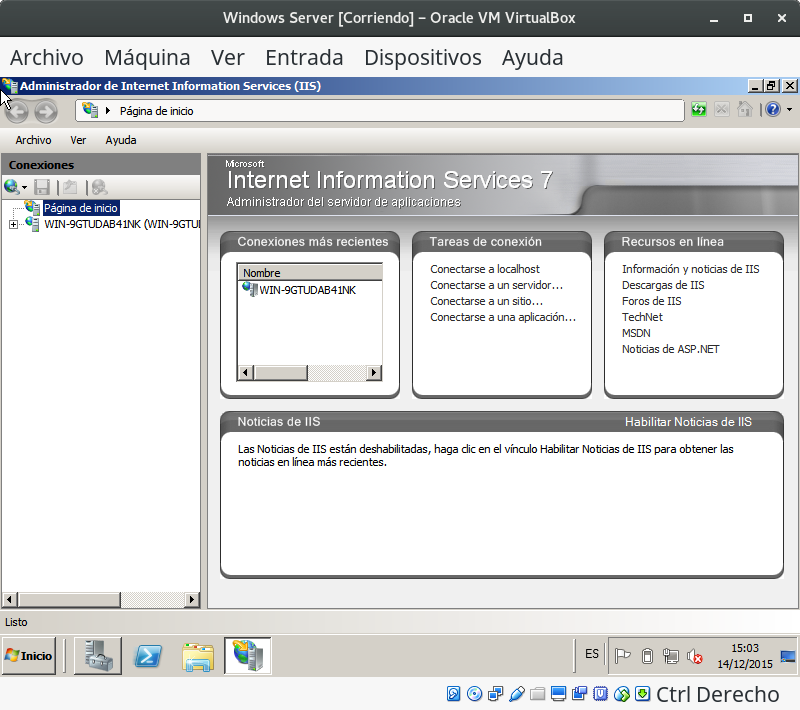
\includegraphics[scale=0.5]{figuras/figura9.png}  %el parámetro scale permite agrandar o achicar la imagen. En el nombre de archivo puede especificar directorios
	
	
	\caption{Administrador de Internet Information Services(ISS)}
	\label{figura9}
\end{figure}

\begin{figure}[H] %con el [H] le obligamos a situar aquí la figura
	\centering
	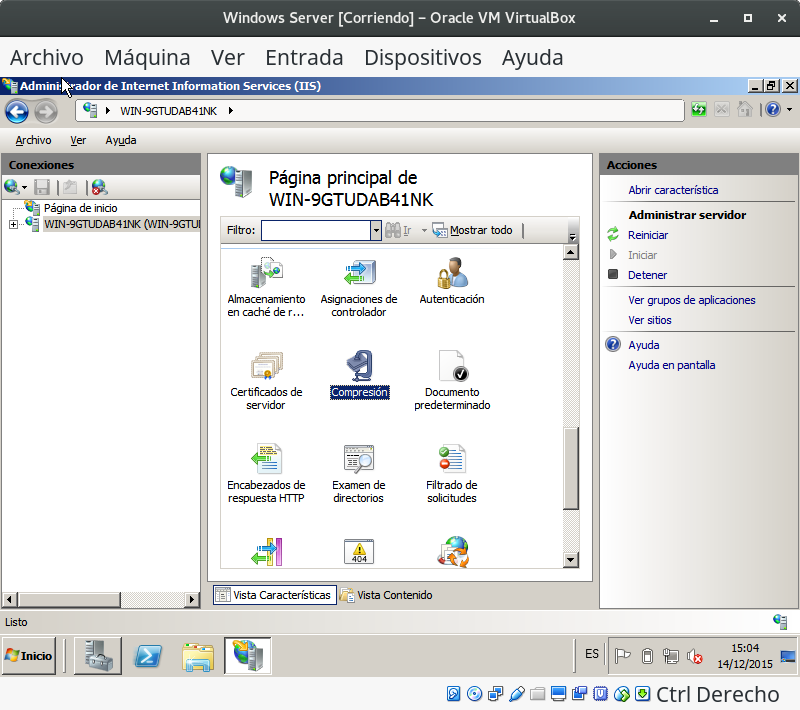
\includegraphics[scale=0.5]{figuras/figura10.png}  %el parámetro scale permite agrandar o achicar la imagen. En el nombre de archivo puede especificar directorios
	
	
	\caption{Compresión}
	\label{figura10}
\end{figure}

\begin{figure}[H] %con el [H] le obligamos a situar aquí la figura
	\centering
	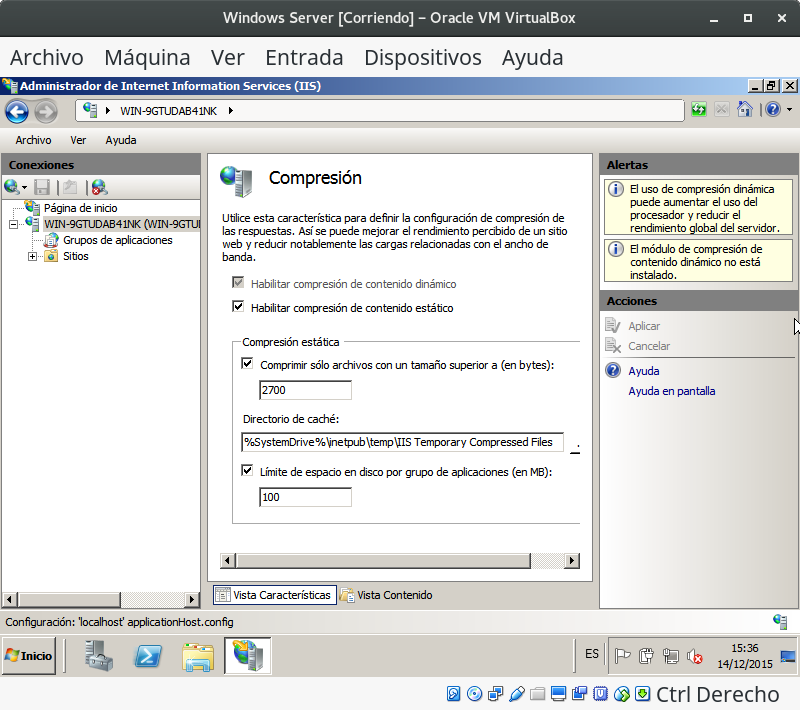
\includegraphics[scale=0.5]{figuras/figura11.png}  %el parámetro scale permite agrandar o achicar la imagen. En el nombre de archivo puede especificar directorios
	
	
	\caption{Valores por defecto de la compresión}
	\label{figura11}
\end{figure}

%%%%%%%%%%%%%%%%%%%%%%%%%%%%%%%%%%%%%%%%%%%%%%%%%%%%
% CUESTIÓN 8
%%%%%%%%%%%%%%%%%%%%%%%%%%%%%%%%%%%%%%%%%%%%%%%%%%%%

\section{Cuestión 8: Usted parte de un SO con ciertos parámetros definidos en la instalación (Práctica 1), ya sabe instalar servicios (Práctica 2) y cómo monitorizarlos (Práctica 3) cuando los somete a cargas (Práctica 4). Al igual que ha visto cómo se puede mejorar un servidor web (Práctica 5 Sección 3.1), elija un servicio (el que usted quiera) y modifique un parámetro para mejorar su comportamiento. (9.b) Monitorice el servicio antes y después de la modificación del parámetro aplicando cargas al sistema (antes y después) mostrando los resultados de la monitorización.}

El parámetro que voy a monitorizar tras realizar un cambio va a ser el tiempo de escritura de distintos tamaños de archivos en dos sistemas distintos sistemas de archivos. Vamos a empezar con un sistema de archivos ext3 y vamos a comprobar si cambiando a ext4 mejora el tiempo de escritura en el mismo.\\
Para el test de carga vamos a utilizar un  script de Python para la escritura de 371 MB en el disco.Después de esto vamos a realizar distintas escrituras de forma paralela de archivos, con otro script de Python.\\

El script de Python para la escritura en disco es el siguiente:

\begin{lstlisting}[language=python]
#!/usr/bin/env python
# -*- coding:utf-8 -*-

from sys import argv
import subprocess

parametros = argv
filename = str(argv[1])
iterations = str(argv[2])
f = open(filename,'w')
for i in range(0,int(iterations),1):
	f.write(str(i))

\end{lstlisting}

El script que crea archivos de distintos tamaños en paralelo que sería el siguiente:\\

\begin{lstlisting}[language=python]
#!/usr/bin/env python
# -*- coding:utf-8 -*-

import sys
import subprocess
import threading 
def script(i):
	subprocess.call(['python','writefile.py','/run/media/pacocp/Paco-Pen/file'+str(i)+'.txt',str(i)])


threads = list()
for i in range(1000,50000,1000):
	t1 = threading.Thread(target=script, args=(i,))
	threads.append(t1)
	t2 = threading.Thread(target=script, args=(i+1000,))
	threads.append(t2)
	t3 = threading.Thread(target=script, args=(i+3000,))
	threads.append(t3)
	if((i+1000)>500000):
		t1.start()
	else:
		if((i+3000)>500000):
			t1.start()
		else:
			t1.start()
			t2.start()
			t3.start()
sys.exit(0)


\end{lstlisting}

Para el test vamos a utilizar un Pen Drive de 32 GB, podemos observarlo con el comando \textbf{sudo fdisk -l} en la Figura \ref{figura12}. Lo vamos a formatear primero   creando la tabla de particiones y a continuación dandole el formato con el programa de creador de discos de KDE, como podemos observar en la Figura \ref{figura14}. Y en la Figura \ref{figura15} podemos observar como tiene formato ext3\\
 
El script que escribe un archivo de 371 MB se ejecutaría con el comando \textbf{time python writefile.py /run/media/pacocp/Pen-Paco/filefirst.txt 50000000} y, como podemos observar en la Figura \ref{figura16}, el tiempo que tarda en escribir es de \textbf{29.7} segundos en \textbf{ext3}.\\

El script que escribe muchos archivos en parello se ejecutaría con el comando \textbf{time python ejercicio8.py} y, como se puede observar en la Figura \ref{figura17}, el tiempo de ejecución es de \textbf{14,79} segundos en ext3.\\

Ahora vamos a proceder a hacer lo mismo, pero esta vez vamos a formatear el pen drive en formato ext4, como podemos observar en la Figura
\ref{figura18}.\\

La ejecución del primer script nos da el resultado de \textbf{28,85} segundos, como podemos observar en la Figura \ref{figura19}.\\
La ejecución del segundo script nos da el resultado de \textbf{14,66} segundos, como podemos observar en la Figura \ref{figura20}.\\

Para verlo de forma más clara y gráfica he creado dos gráficas de los tiempos que podemos observar en las Figuras \ref{figura21} y \ref{figura22}. Podemos observar la clara diferencia de mejora en tiempos en las dos gráficas. Claro que si vemos números no hay tanto diferencia por ejemplo entre \textbf{14,79} y \textbf{14,66}, pero si tenemos que realizar muchas escrituras en disco, ahorraremos muchísimo tiempo gracias al pequeño que vamos ahorrando en cada una, lo que supone una mejora en nuestro sistema.

\begin{figure}[H] %con el [H] le obligamos a situar aquí la figura
	\centering
	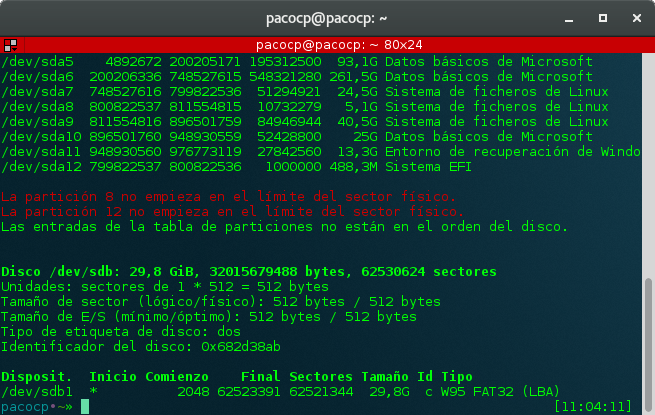
\includegraphics[scale=0.5]{figuras/figura12.png}  %el parámetro scale permite agrandar o achicar la imagen. En el nombre de archivo puede especificar directorios
	
	
	\caption{Resultado de \textbf{sudo fdisk -l}}
	\label{figura12}
\end{figure}

\begin{figure}[H] %con el [H] le obligamos a situar aquí la figura
	\centering
	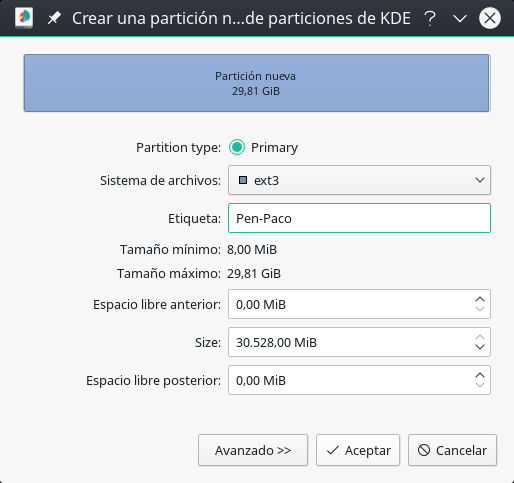
\includegraphics[scale=0.5]{figuras/figura14.png}  %el parámetro scale permite agrandar o achicar la imagen. En el nombre de archivo puede especificar directorios
	
	
	\caption{Lo formateamos en formato ext3}
	\label{figura14}
\end{figure}

\begin{figure}[H] %con el [H] le obligamos a situar aquí la figura
	\centering
	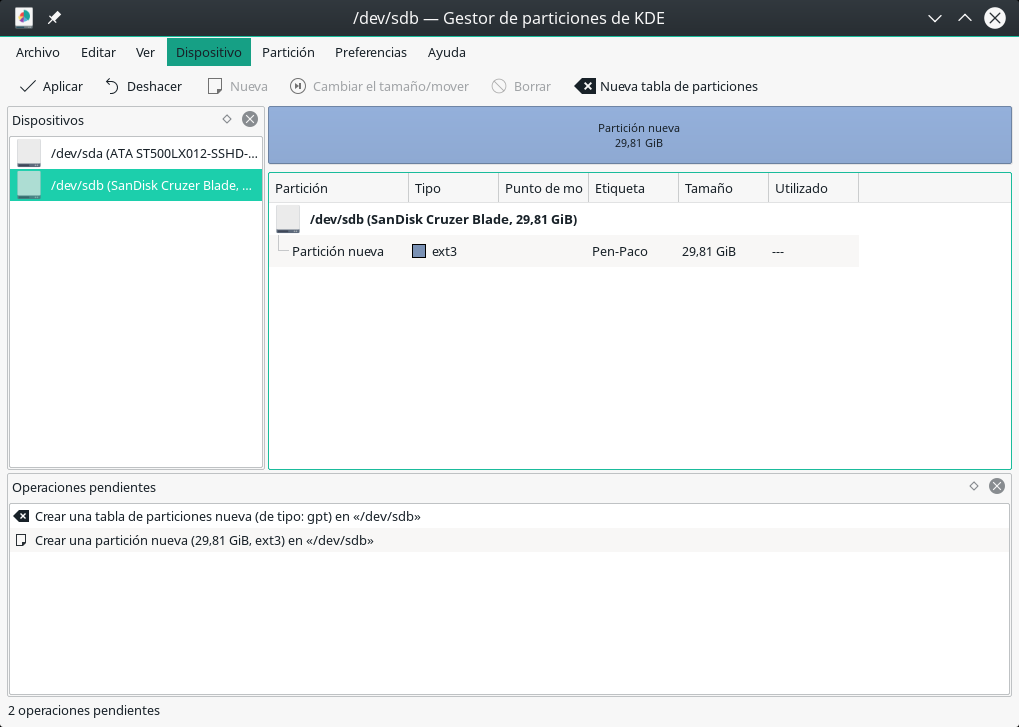
\includegraphics[scale=0.3]{figuras/figura15.png}  %el parámetro scale permite agrandar o achicar la imagen. En el nombre de archivo puede especificar directorios
	
	
	\caption{Vemos que está en formato ext3}
	\label{figura15}
\end{figure}

\begin{figure}[H] %con el [H] le obligamos a situar aquí la figura
	\centering
	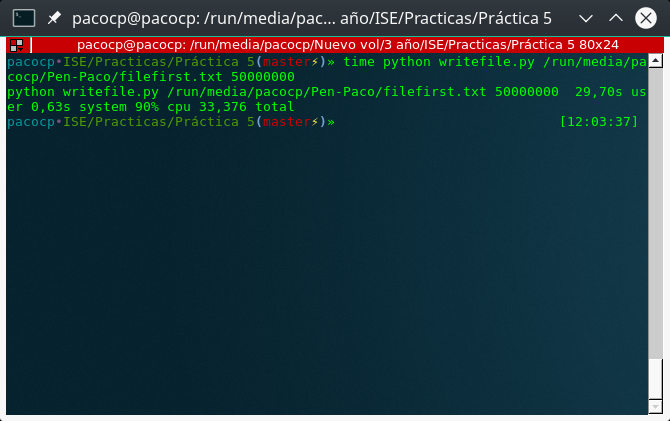
\includegraphics[scale=0.5]{figuras/figura16.png}  %el parámetro scale permite agrandar o achicar la imagen. En el nombre de archivo puede especificar directorios
	
	
	\caption{Ejecución del script de Python para la escritura de 371 MB en \textbf{ext3}}
	\label{figura16}
\end{figure}

\begin{figure}[H] %con el [H] le obligamos a situar aquí la figura
	\centering
	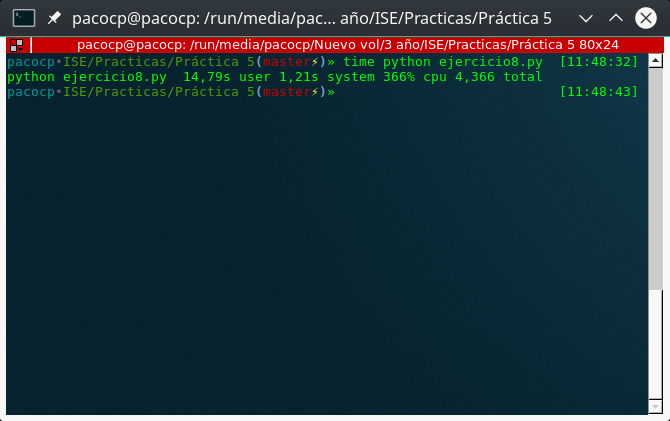
\includegraphics[scale=0.5]{figuras/figura17.png}  %el parámetro scale permite agrandar o achicar la imagen. En el nombre de archivo puede especificar directorios
	
	
	\caption{Ejecución del script de Python para la escritura en paralelo en \textbf{ext3}}
	\label{figura17}
\end{figure}

\begin{figure}[H] %con el [H] le obligamos a situar aquí la figura
	\centering
	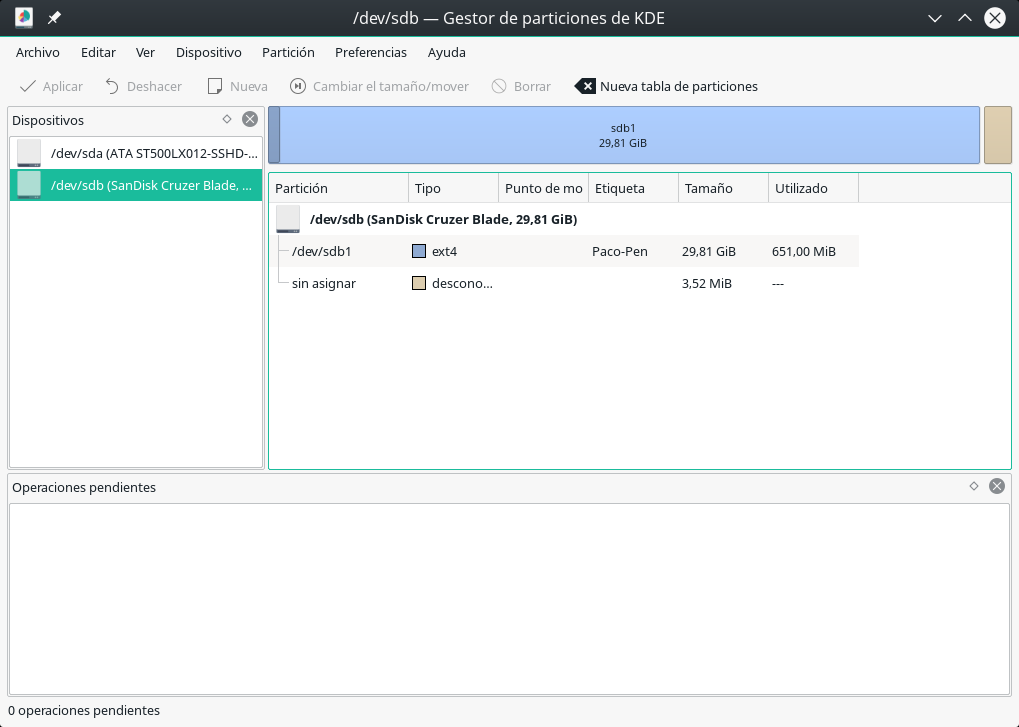
\includegraphics[scale=0.35]{figuras/figura18.png}  %el parámetro scale permite agrandar o achicar la imagen. En el nombre de archivo puede especificar directorios
	
	
	\caption{Formateado el pen drive en formato \textbf{ext4}}
	\label{figura18}
\end{figure}

\begin{figure}[H] %con el [H] le obligamos a situar aquí la figura
	\centering
	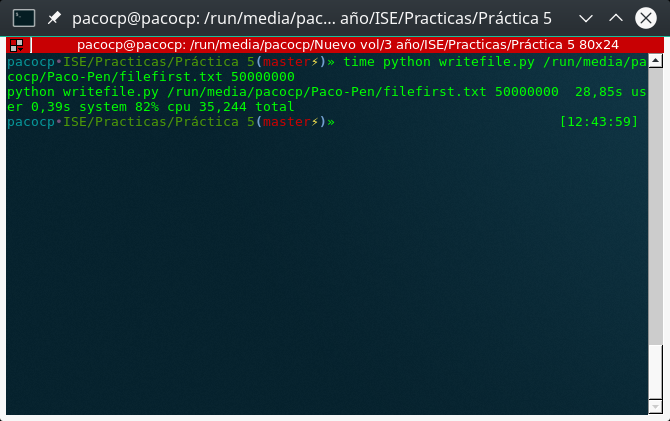
\includegraphics[scale=0.5]{figuras/figura19.png}  %el parámetro scale permite agrandar o achicar la imagen. En el nombre de archivo puede especificar directorios
	
	
	\caption{Ejecución del script de Python para la escritura de 371 MB en \textbf{ext4}}
	\label{figura19}
\end{figure}

\begin{figure}[H] %con el [H] le obligamos a situar aquí la figura
	\centering
	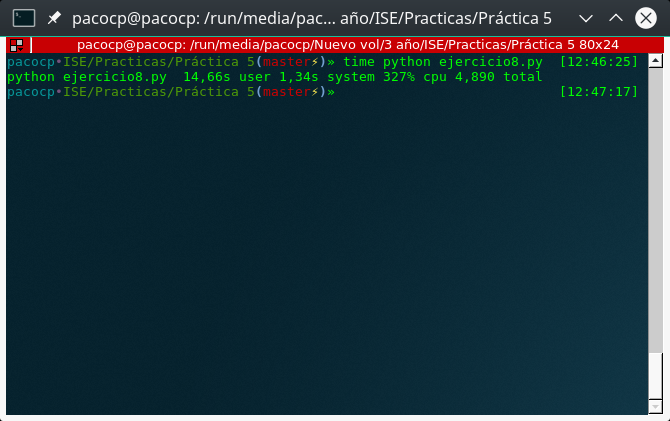
\includegraphics[scale=0.5]{figuras/figura20.png}  %el parámetro scale permite agrandar o achicar la imagen. En el nombre de archivo puede especificar directorios
	
	
	\caption{Ejecución del script de Python para la escritura en paralelo en \textbf{ext4}}
	\label{figura20}
\end{figure}

\begin{figure}[H] %con el [H] le obligamos a situar aquí la figura
	\centering
	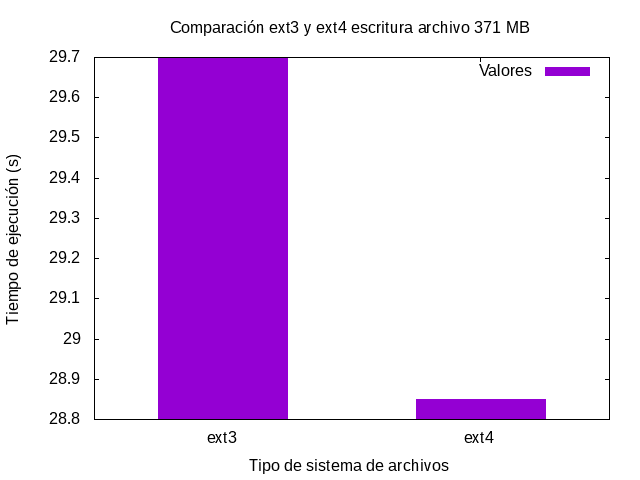
\includegraphics[scale=0.5]{figuras/figura21.png}  %el parámetro scale permite agrandar o achicar la imagen. En el nombre de archivo puede especificar directorios
	
	
	\caption{Gráfica comparación escritura de 371 MB}
	\label{figura21}
\end{figure}

\begin{figure}[H] %con el [H] le obligamos a situar aquí la figura
	\centering
	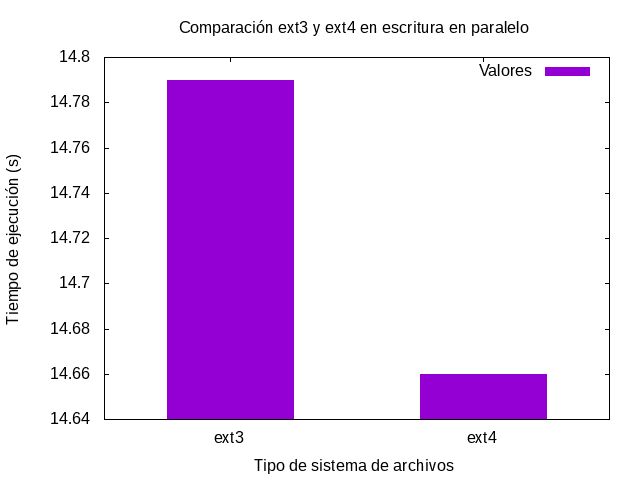
\includegraphics[scale=0.5]{figuras/figura22.png}  %el parámetro scale permite agrandar o achicar la imagen. En el nombre de archivo puede especificar directorios
	
	
	\caption{Gráfica comparación escritura de archivos en paralelo}
	\label{figura22}
\end{figure}
\newpage
\bibliography{citas} %archivo citas.bib que contiene las entradas 
\bibliographystyle{ieeetr} % hay varias formas de citar
\end{document}